%%%%%%%%%%%%%%%%%%%%%%%%%%%%%%%%%%%%%%%%%%%%%%%%%%%%%%%%%%%%
%%% ELIFE ARTICLE TEMPLATE
%%%%%%%%%%%%%%%%%%%%%%%%%%%%%%%%%%%%%%%%%%%%%%%%%%%%%%%%%%%%
%%% PREAMBLE 
\documentclass[9pt,lineno]{elife}
% \documentclass{article}

% \usepackage{arxiv}

\usepackage[utf8]{inputenc} % allow utf-8 input
\usepackage[T1]{fontenc}    % use 8-bit T1 fonts
\usepackage{hyperref}       % hyperlinks
\usepackage{url}            % simple URL typesetting
\usepackage{booktabs}       % professional-quality tables
\usepackage{amsmath}
\usepackage{amsthm}
% \usepackage{amssymb}
\usepackage{mathtools}
\usepackage{amsfonts}       % blackboard math symbols
\usepackage{nicefrac}       % compact symbols for 1/2, etc.
\usepackage{microtype}      % microtypography
\usepackage{graphicx}
\usepackage{comment}
\usepackage{siunitx}
\usepackage{algorithm}
% \usepackage{lineno}
% \linenumbers
\usepackage[noend]{algpseudocode}
%\usepackage[style=nature]{biblatex}
% \AtEveryBibitem{\clearlist{language}}
% argmax operator
\DeclareMathOperator*{\argmax}{argmax}
% \addbibresource{references.bib}

%%%%%%%%%%%%%%%%%%%%%%%%%%%%%%%%%%%%%%%%%%%%%%%%%%%%%%%%%%%%
%%% ARTICLE SETUP
%%%%%%%%%%%%%%%%%%%%%%%%%%%%%%%%%%%%%%%%%%%%%%%%%%%%%%%%%%%%
\title{Bayesian machine learning analysis of single-molecule fluorescence colocalization images}
% Bayesian classification of single-molecule fluorescence colocalization images
% Bayesian analysis of single-molecule fluorescence colocalization images

\author[1]{Yerdos A. Ordabayev}
\author[1]{Larry  J. Friedman}
\author[1*]{Jeff Gelles}
\author[1*]{Douglas L. Theobald}
\affil[1]{Department of Biochemistry, Brandeis University, Waltham, MA 02454 USA}

\corr{gelles@brandeis.edu}{JG}
\corr{dtheobald@brandeis.edu}{DLT}

% \author{Yerdos A. Ordabayev\and Larry  J. Friedman\and Jeff Gelles\thanks{Corresponding authors: gelles@brandeis.edu and dtheobald@brandeis.edu}\and Douglas L. Theobald\footnotemark[1] \\ Department of Biochemistry, Brandeis University, Waltham, MA 02454 USA}

%%%%%%%%%%%%%%%%%%%%%%%%%%%%%%%%%%%%%%%%%%%%%%%%%%%%%%%%%%%%
%%% ARTICLE START
%%%%%%%%%%%%%%%%%%%%%%%%%%%%%%%%%%%%%%%%%%%%%%%%%%%%%%%%%%%%

\begin{document}

\maketitle

\begin{abstract} % 150 words limit
Multi-wavelength single-molecule fluorescence colocalization (CoSMoS) methods allow elucidation of complex biochemical reaction mechanisms. However, analysis of CoSMoS data is intrinsically challenging because of low image signal-to-noise ratios, non-specific surface binding of the fluorescent molecules, and analysis methods that require subjective inputs to achieve accurate results. Here, we use Bayesian probabilistic programming to implement Tapqir, an unsupervised machine learning method based on a holistic, physics-based causal model of CoSMoS data.  This method accounts for uncertainties in image analysis due to photon and camera noise, optical non-uniformities, non-specific binding, and spot detection. Rather than merely producing a binary ``spot/no spot'' classification of unspecified reliability, Tapqir objectively assigns spot classification probabilities that allow accurate downstream analysis of molecular dynamics, thermodynamics, and kinetics.   We both quantitatively validate Tapqir performance against simulated CoSMoS image data with known properties and also demonstrate that it implements fully objective, automated analysis of experiment-derived data sets with a wide range of signal, noise, and non-specific binding characteristics. 
\end{abstract}

% 2500-3500 limit
% wc 7925 - 7006 = 919
\section*{Introduction}

%Nature Methods says: To enhance the practical relevance of each paper, description of the method must be accompanied by its validation, its application to an important biological question and results illustrating its performance in comparison to available approaches. Articles are selected for publication that present broad interest, thorough assessments of methodological performance and comprehensive technical descriptions that facilitate immediate application.

A central concern of modern biology is understanding at the molecular level the chemical and physical mechanisms by which protein and nucleic acid macromolecules  perform essential cellular functions.  The operation of many such macromolecules requires that they work not as isolated molecules in solution but as components of dynamic molecular complexes that self-assemble and change structure and composition as they function.  For more than  two decades, scientists have successfully explored the molecular mechanisms of many such complex and dynamic systems using multi-wavelength single molecule fluorescence methods such as smFRET (single-molecule fluorescence resonance energy transfer) \cite{Roy2008-fo} and single-molecule colocalization methods like CoSMoS (colocalization single molecule spectroscopy) \cite{Larson2014-os, Van_Oijen2011-ig}.

CoSMoS is a technique to measure the kinetics of dynamic interactions between individual molecules.  The CoSMoS method has been used for elucidating the mechanisms of complex biochemical processes \textit{in vitro}. Examples include cell cycle regulation \cite{Lu2015-eu}, ubiquitination and proteasome-mediated protein degradation \cite{Lu2015-jq}, DNA replication \cite{Geertsema2014-bt,Ticau2015-ib}, transcription \cite{Zhang2012-no,Friedman2012-if,Friedman2013-sf}, micro-RNA regulation \cite{Salomon2015-kq}, pre-mRNA splicing \cite{Shcherbakova2013-bi, Krishnan2013-fy, Warnasooriya2014-ls}, ribosome assembly \cite{Kim2014-zc}, translation \cite{Wang2015-tt,Tsai2014-mi,OLeary2013-wo}, signal recognition particle-nascent protein interaction \cite{Noriega2014-vj}, and cytoskeletal regulation \cite{Smith2013-qj,Breitsprecher2012-mj}. 

Fig. 1a illustrates an example CoSMoS experiment to measure the interaction kinetics of RNA polymerase molecules with DNA. In the experiment \cite{Rosen2020-zn}, we first measured the locations of individual DNA molecules (the ``targets'') tethered to the surface of an observation chamber at low density. Next, a solution containing RNA polymerase II molecules (the ``binders'') was added to the solution over the surface and the chamber surface was imaged by TIRF (total internal reflection fluorescence) microscopy. When the binder molecules are freely diffusing in solution, they are not visible in TIRF. In contrast, when bound to a target, a single binder molecule is detected as a discrete fluorescent spot colocalized with the target position \cite{Friedman2006-kb, Friedman2015-nx}.

Effective data analysis is a major challenge in the use of the CoSMoS technique. The basic goal is to acquire information at each time point about whether a binder molecule fluorescence spot is observed at the image position of a target molecule (e.g., whether a colocalized green RNA polymerase is observed at the surface location of a blue DNA spot in Fig. 1b). Although CoSMoS images are conceptually simple -- they consist only of diffraction-limited fluorescent spots collected in several wavelength channels -- efficient analysis of the images is inherently challenging. The number of photons emitted by a single fluorophore is limited by fluorophore photobleaching. Consequently, it is desirable to work at the lowest feasible excitation power in order to maximize the duration of experimental recordings and to efficiently capture relevant reaction events. Achieving higher time resolution divides the number of emitted photons between a larger number of images, so that photon shot noise ordinarily dominates the data statistics. Furthermore, the required concentrations of binder molecules can sometimes create significant background noise \cite{Peng2018-ge, Van_Oijen2011-ig}, even with zero-mode waveguide instruments \cite{Chen2014-jd}. These technical difficulties result in CoSMoS images that frequently have low signal-to-noise ratios (SNR), making discrimination of real fluorescent spots from noise a significant challenge. Also, there are usually non-specific interactions of the binder molecule with the chamber surface, and these artefacts can give rise to both false positive and false negative spot detection. These defects in analyzing spot colocalization interfere with the interpretation of CoSMoS data to measure reaction thermodynamics and kinetics and to infer molecular mechanisms.

Most CoSMoS spot detection methods are based on integrating the binder fluorescence intensity over small regions of the image  centered on the location of individual target molecules, and then using crossings of an intensity threshold to score binder molecule arrival and departure \cite{Friedman2015-nx}. However, integration discards data about the spatial distribution of intensity that can (and should) be used to distinguish authentic on-target spots from artefacts caused by noise or off-target binding.  More recently, improved methods \cite{Friedman2015-nx,Smith2019-yb} were developed that directly analyze TIRF images, using the spatial distribution of binder fluorescence intensity around the target molecule location. All of these methods, whether image- or integrated intensity-based, make a binary decision about the presence or absence of a binder spot at the target location.  Treating all binary decisions as equal neglects differences in the confidence of each spot detection decision caused by variations in noise, signal intensity, and non-specific binding.  Failure to account for spot confidence decreases the reliability of downstream thermodynamic and kinetic analysis.

In this paper, we describe a qualitatively different method for analysis of CoSMoS data implemented in a computer program, Tapqir (Kazakh: clever or inventive; pronunciation: \emph{tap-keer}). Tapqir analyzes 2-D image data, not integrated intensities.  Unlike prior methods, our approach is based on an explicit, global model for CoSMoS image formation and uses Bayesian inference to determine the values of model parameters and their associated uncertainties. The model includes realistic shot noise in fluorescent spots and background, camera noise, the size and shape of spots, and the presence of both target-specific and nonspecific binder molecules in the images. Most importantly, instead of yielding a binary spot-/no-spot determination, the algorithm calculates the probability of a target-specific spot being present at each time point and target location. The calculated probability can then be used in subsequent analyses of the molecular thermodynamics and kinetics. Unlike alternative approaches, Tapqir does not use subjective threshold settings so it can be used effectively and accurately by non-expert practitioners. The program is implemented in the Python-based probabilistic programming language Pyro \cite{Bingham2019-qy}, which facilitates modification of the global model and efficient use of graphics processing unit (GPU)-based hardware for rapid parallel processing of data. 

% wc 2992 ->  6980-3988
\section{Results}

\subsection{The Model}

In this work, we present a probabilistic generative model for single-molecule image-data and describe Bayesian inference approach used to obtain posterior distributions of latent model parameters. The generative model can be interpreted as a causal process that produces the observed image data. The graphical model in Figure 2A visually describes latent variables of the model and conditional independence structure of the model. We model the observed image as ``spot'' images of binder molecules superimposed on background image. Fluorescence spots are modeled as a 2D Gaussians parameterized by a set of variables ($h, w, x, y$) which accurately approximates fluorescence microscope point spread function \cite{Zhang2007-rb}. The model depends on various unobserved physical parameters such as background photon intensity and the number, position, shape, and intensity of each spot in the image. The unobserved parameters, in turn, are described by prior distributions which embed into the model our existing knowledge of the experiment, such as the likely position of an on-target spot. Explicitly model on-target and off-target spots.

Our model assumes that at maximum 2 spots in total can be present in a single image and at maximum only one on-target spot. The image model described above allows to capture many of the characteristics of real experimental data, such as site and time dependent fluctuations in the local background signal, time dependent fluctuations in the spot intensity and its position, simultaneous binding of on-target and off-target spots, Gamma distributed noise, which is more realistic than Gaussian noise. Figure 2B,C,D shows examples where there is no spot, one spot, or two spots and corresponding spot parameters in the table.

Total observed intensity is the sum of the offset signal (dark current) plus the photon counts amplified by the gain setting of the camera. The linear relationship between the noise variance and the mean intensity is built into the intensity model through the gain and offset parameters and the gain parameter is fitted along with other parameters. Distribution of the offset signal is obtained as a histogram density signal from the single-molecule images (Figure ).  In Figure we show raw images and their intensity distributions along with the images simulated from the posterior distribution (posterior predictive checking). Comparison of images and distributions for spot/no spot cases show that our model accurately models intensity as a function of mean intensity reflecting the dependence of the noise on the mean intensity. Additionally, Figure shows that the gain parameter is accurately inferred for a simulated set of data with varying gain parameter where the true value of the gain parameter is known.

\subsection{Bayesian Inference and Implementation}

Posterior distributions of latent variables conditioned on the observed data is given by the Bayes' theorem. The evidence in general is intractable. Here we use stochastic variational inference (SVI) approach and maximize the evidence-lower bound (ELBO). Our program Tapqir is open-source (github link) and is implemented in the probabilistic programming language Pyro. The advantage of using PPL like Pyro is its black box SVI approach which allows to focus on the model, efficient computation on GPU, scalability to large datasets. Details of the generative model and variational model are given in the online Methods section.

\subsection{Analysis of simulated data}

As a validation of our model we demonstrate its application to simulated synthetic data. Fake-data simulation is important because it allows to directly check that the inference on latent variables is reliable. Thus, fake-data simulation provides an upper bound of what can be learned reliably about the model for various types of data. Simulation parameters details are described in the online Methods. We made 10 randomized simulations and then fit the synthetic data to the model. Figure 3 shows plots of the simulated values of the global parameters (gain, average on-target spot probability, average off-target spot probability, proximity) vs the fitted values. The results demonstrate that model parameters can be reliably recovered which is good.

MCC plot. Example traces.

\subsection{Analysis of experimental data}

Thermodynamic Analysis.

In this section, we describe different aspects of our model. The Bayesian model described here is holistic in a sense that the observed data and all of the model parameters are interconnected. However, its modular structure allows to view and analyze different parts of the model separately. Below we review briefly the CoSMoS method and the type of data generated by CoSMoS experiments, and then describe the image model, the intensity model, spot-detection, and co-localization aspects of the model.

\subsection{Multi-wavelength single-molecule co-localization methods}

Before describing the approach used for the analysis of CoSMoS data, it is helpful to  review briefly the experimental method. The key features of a CoSMoS experiment include: 1) One species of fluorescently labeled molecule (called the “target”) is tethered to the surface of the observation chamber. Target molecules are immobilized at a surface density sufficiently low that the mean nearest-neighbor distance is large relative to the point-spread function (i.e., the diffraction-limited spot size) of the microscope. 2) Molecules, each species labeled with a different dye color, are added to the solution over the surface, typically at concentrations $\leq 1 \mu$M. When these “binder” molecules are freely diffusing in solution, they are invisible in TIRF. In contrast, when they are bound to the target, single binder molecules are detected as discrete fluorescent spots (Figure \ref{fig:cosmos_experiment}). The combination of features 1 and 2 means that formation of an individual binder-target complex is detected as spot appearance; dissociation of a binder-target complex is detected as spot disappearance \cite{Friedman2006-kb, Friedman2015-nx}.

\subsection{CoSMoS image data}

CoSMoS data analysis requires identifying the locations of target molecules and the corresponding positions in the binder molecule camera channel. Image pre-processing steps include alignment of images from multiple wavelength channels and drift correction \cite{Friedman2015-nx, Smith2019-yb}. Single-molecule images after pre-processing steps consists of a $P \times P$ matrix of pixel intensities with the target molecule at the center of the image. One experiment typically consists of a set of images where we have $N$ target sites ($n \in \{1,\dots,N\}$) each consisting of a series of $F$ different images in a recording ($f \in \{1,\dots,F\}$) (a “recording”).

CoSMoS images consist of offset signal, background intensity and diffraction-limited spots. Detection of on-target binding depends on the intensity of the spot and its distance to the target molecule. The size $P=14$ of the selected area is chosen to be large enough to detect the on-target spot and reliably determine the local background intensity. In addition to the on-target spot, non-specifically bound binder molecules can also be present in the image. Usually no more than two spots are present in the single image. Frequently, identification of on-target binding is complicated by molecules binding off-target which distort the shape of the on-target spot and its apparent distance to the target. 

%\begin{figure}
%\includegraphics[width=\linewidth]{figures/figure1.jpg}
%\caption{Co-localization single molecule spectroscopy experiment. (A) Target molecules are localized in the blue channel and then on-target and off-target areas of interest are selected. (B) Movies of the binder molecule collected in the green channel. In selected AoI binder molecules can be on-target, off-target, or absent.}
%\label{fig:cosmos_experiment}
%% If the optional argument in the square brackets is "none", then the caption *will not appear in the main figure at all* and only the full caption will appear under the supplementary figure at the end of the manuscript.
%\figsupp[Shorter caption for main text.]{This is a supplementary figure's full caption, which will be used at the end of the manuscript.}{\includegraphics[width=6cm]{frog}}\label{figsupp:sf1}
%\figsupp{This is another supplementary figure.}{\includegraphics[width=6cm]{frog}}
%\figdata{This is a description of a data source.}\label{figdata:first}
%\figdata{This is another description of a data source.}\label{figdata:second}
%\end{figure}

%\begin{figure}
%\includegraphics[width=\linewidth]{figures/figure3a.png}
%\includegraphics[width=\linewidth]{figures/figure3b.png}
%\includegraphics[width=\linewidth]{figures/figure3c.png}
%\caption{Co-localization single molecule spectroscopy experiment. (A) Target molecules are localized in the blue channel and then on-target and off-target areas of interest are selected. (B) Movies of the binder molecule collected in the green channel. In selected AoI binder molecules can be on-target, off-target, or absent.}
%\label{fig:view}
%\end{figure}

\subsection{Image Model Module} 

We model the observed image as ``spot'' images of binder molecules superimposed on background image. In particular, background image consists only of constant background intensity $\mathrm{b}_{nf}$ that can vary from image to image. Our model assumes that at maximum $K=2$ number of spots can be present in a single image.  Fluorescence spot is modeled as a 2D Gaussian which accurately approximates fluorescence microscope point spread function \cite{Zhang2007-rb}. Each spot is parameterized by integrated scalar intensity $\mathrm{h}_{nfk}$, width $\mathrm{w}_{nfk}$, and relative position $\mathrm{x}_{nfk}$ and $\mathrm{y}_{nfk}$ to the target molecule. All of the spot parameters are local/individual for each spot.

We use binary indicator variable $\mathbf{m} = \{\mathrm{m}_{nfk}\}$ to denote the presence of each individual spot ($k \in \{1,\dots,K\}$). The value of the index variable $\theta_{nf} \in \{0,1,\dots,K\}$ specifies the index of the on-target spot when it is present and equals zero when the on-target spot is absent. There are $2^K + K2^{K-1}$ unique combinations of $\mathrm{m}$ and $\theta$ which define the state space for each image. Table~\ref{tab:states} shows the state space when $K=2$. Thus, we get the image model ($\mu^I_{nfij}$) calculated as the sum of the background intensity ($\mathrm{b}_{nf}$) and 2D Gaussian spots ($\mu^S_{knfij}$) present in the image.

\subsection{Spot Detection}

WIP

Spot detection is performed in a probabilistic manner. Spot existence probability depends on the information in the entire image. However, it primarily correlates with the intensity of the spot. Discrimination of spots from random fluctuations in the background signal depends on the prior and not on the threshold parameter. In the absence of prior information uninformative prior can be used. Plotting results show that with half normal prior spots have to be roughly above 1 SNR.

\subsection{Co-localization}

For the spots that are present in the image they can be further classified as on-target (co-localization) or off-target (non-specific). The probability of being on-target or off-target is dictated primarily by the distance to the target. Spots bound on-target and off-target have different prior distributions of their location relative to the target molecule. This prior knowledge is used to discriminate between on- and off-target spots in a probabilistic manner using mixture distributions model. Off-target spots have a uniform prior distribution across the image and can bind anywhere on the surface with equal probability. On-target spots, on the other hand, are clustered near the target molecule. Standard deviation of the distribution of on-target spots depends on the spot localization accuracy and the mapping accuracy between target and binder channels (?). By analyzing simulated data we have established that this parameter, also called the proximity parameter, can be reliably determined by floating it during the fit (Figure ). Alternatively, proximity parameter can be determined experimentally and fixed in the model. Figure show the distribution of the center of mass of on-target spots which are tightly clustered around the target molecule. On the other hand, off-target spots are distributed more uniformly across the area of the image.

Second, the posterior probabilities of being classified as on-target or off-target spot depends on the prior average frequencies of on-target and off-target spots. Increasing the ratio of the off-target molecules to on-target molecules decreases the probability of the spot being on-target reflecting the fact that.

This standard distribution can be determined independently and used as a fixed parameter in the model. However, it can also be floated in the fit and determined from the overall distribution of the center of masses of spots. $\sigma^{xy}$, $\pi^z$, and $\lambda^j$ are correlated. Figure shows simulated data with varying parameters where the true values of parameters are inferred correctly. Note that the posterior probability of the spot class depends on its relative position to the target and average probabilities of on-target and off-target spots.

\subsection{Informal Kinetic/Thermodynamic Analysis}

WIP

% wc 790
\section{Discussion}

\lipsum[9]

\section*{Methods}

\subsection*{Probabilistic model for the CoSMoS image data} 

Our intent is to model CoSMoS image data by accounting for the most significant physical aspects of the image generation process, in particular a realistic description of photon noise, using model parameters that likewise reflect underlying physical factors known to affect the experimental setup. We use a mixture model to detect binder molecules that are present in the image and to distinguish between specifically and non-specifically bound molecules. An extended version of the graphical representation of the model for CoSMoS data that includes probability distributions is shown in Extended Data Fig. 1a. The corresponding generative model represented as pseudocode is shown in Algorithm 1. Below we describe the model in detail starting with the observed data and the likelihood function and then proceed with model parameters and their prior distributions.

\subsubsection*{Observed data and likelihood function}

Microscope image preprocessing gives a list of drift-corrected locations of the target molecules in each frame with sub-pixel accuracy. Based on this information, we select $P \times P$-pixel AOIs centered with pixel resolution at the target location. The observed data ($D$) thus consists of a set of $P \times P$ grayscale values of pixel intensity as measured by the camera in arbitrary units, collected at $N$ number of AOI sites for a range of $F$ number of frames:
%
\begin{subequations}
\begin{align}
    D &\in \mathbb{R}_{>0}^{\mathsf{AOI}[N] \times \mathsf{frame}[F] \times \mathsf{pixelX}[P] \times \mathsf{pixelY}[P]} \\
    x_c &\in [-1/2, 1/2]^{\mathsf{AOI}[N] \times \mathsf{frame}[F]} \\
    y_c &\in [-1/2, 1/2]^{\mathsf{AOI}[N] \times \mathsf{frame}[F]}
\end{align}
\end{subequations}

\noindent
where $x_c$ and $y_c$ are the coordinates of the target molecule relative to the center of the AOI. While experimental intensity measurements are integers we treat them as continuous values in our analysis.

We model the data $D$ as the sum of a fixed photon-independent offset $\delta$ introduced by the camera and the noisy photon-dependent pixel intensity values $I$.
%
\begin{subequations}
\begin{align}
    \delta &\in \mathbb{R}_{>0}^{\mathsf{AOI}[N] \times \mathsf{frame}[F] \times \mathsf{pixelX}[P] \times \mathsf{pixelY}[P]} \\
    I &\in \mathbb{R}_{>0}^{\mathsf{AOI}[N] \times \mathsf{frame}[F] \times \mathsf{pixelX}[P] \times \mathsf{pixelY}[P]} \\ 
    D &= \delta + I
\end{align}
\end{subequations}

In our model, each pixel in the photon-dependent image $I$ has a  variance which is equal to  the mean intensity $\mu^I$ of that pixel multiplied by the gain $g$. This formulation accounts for both photon shot noise and additional noise introduced by EMCCD camera amplification (ref). We model the intensity $I$ using a continuous Gamma distribution as the likelihood function:
%
\begin{equation}
    I \sim \mathbf{Gamma} (\mu^I, \sqrt{\mu^I \cdot g})
\end{equation}

The parameterization of the Gamma distribution (and all other distributions we use in this work) is given in Extended Data Table 2.

\subsubsection*{Image model}

The mean of the photon-dependent pixel intensity $\mu^I$ is represented  as the sum of a background intensity $b$ and the intensities from fluorescence spots modeled as  2-dimensional Gaussians $\mu^S$ 
%
\begin{subequations}
\begin{align}
    \mu^I &\in \mathbb{R}_{>0}^{\mathsf{AOI}[N] \times \mathsf{frame}[F] \times \mathsf{pixelX}[P] \times \mathsf{pixelY}[P]} \\
    b &\in \mathbb{R}_{>0}^{\mathsf{AOI}[N] \times \mathsf{frame}[F]} \\
    m &\in \{ 0, 1 \}^{\mathrm{spot}[K] \times \mathsf{AOI}[N] \times \mathsf{frame}[F] } \\
    \mu^I &= b + \sum_{\mathsf{spot}[K]} m \odot{} \mu^S
\end{align}
\end{subequations}

\noindent
where $\odot$ is an element-wise product operation. For simplicity we allow at most $K$ spots in each frame of each AOI.  (In this article, we always use $K$ equal to 2.)  The presence of a given spot in the image is encoded in the binary spot existence parameter $m$, where $m = 1$ when the corresponding spot is present and $m = 0$ when it is absent. The background $b$ is local to each frame in each AOI and is restricted to positive values.



The intensities for a 2-dimensional Gaussian spot centered at ($x$, $y$) are defined for each pixel coordinate ($i$, $j$):
%
\begin{subequations}
\begin{align}
    i &\in \{-(P-1)/2, \dots, (P-1)/2\}^{\mathsf{pixelX}[P]} \\
    j &\in \{-(P-1)/2, \dots, (P-1)/2\}^{\mathsf{pixelY}[P]} \\
    \mu^S &\in \mathbb{R}_{>0}^{\mathsf{spot}[K] \times \mathsf{AOI}[N] \times \mathsf{frame}[F] \times \mathsf{pixelX}[P] \times \mathsf{pixelY}[P]}  \\
    \mu^S &= \dfrac{h}{2 \pi \cdot w^2} \exp{\left( -\dfrac{(i-x)^2 + (j-y)^2}{2 \cdot w^2} \right)}
\end{align}
\end{subequations}

\noindent
with parameters total integrated intensity $h$, width $w$, and center ($x$, $y$). Spatial coordinates $x$, $y$, $i$, and $j$ are taken relative to the AOI center. 
%
\begin{subequations}
\begin{align}
    h &\in \mathbb{R}_{>0}^{\mathsf{spot}[K] \times \mathsf{AOI}[N] \times \mathsf{frame}[F]} \\
    w &\in \mathbb{R}_{>0}^{\mathsf{spot}[K] \times \mathsf{AOI}[N] \times \mathsf{frame}[F]} \\
    x &\in \mathbb{R}^{\mathsf{spot}[K] \times \mathsf{AOI}[N] \times \mathsf{frame}[F]} \\
    y &\in \mathbb{R}^{\mathsf{spot}[K] \times \mathsf{AOI}[N] \times \mathsf{frame}[F]}
\end{align}
\end{subequations}

To discriminate between spots from target-specific and target-nonspecific binding, we use the index parameter $\theta$ to specify the index of the target-specific spot when it is present and use zero when no target-specific spot is present.
%
\begin{equation}
    \theta \in \{ 0, 1, \dots, K \}^{ \mathsf{AOI}[N] \times \mathsf{frame}[F] }
\end{equation}

Probability of target-specific spot presence is calculated as

\begin{equation}
    p(\mathsf{specific}) = p(\theta > 0)
\end{equation}

\subsubsection*{Prior distributions}

The prior distributions for the unobserved model parameters are detailed below and illustrated in Extended Data Fig. 1a. Unless otherwise indicated we assume largely uninformative priors (such as the Half-Normal distribution with large mean). Parameters of prior distributions can be changed if necessary.
%
\begin{enumerate}
    \item Background intensity is modeled using a hierarchical Gamma prior
%
\begin{subequations}
\begin{align}
    \mu^b &\in \mathbb{R}_{>0}^{\mathsf{AOI}[N]} \\
    \sigma^b &\in \mathbb{R}_{>0}^{\mathsf{AOI}[N]} \\
    b &\sim \mathbf{Gamma}(\mu^b, \sigma^b)
\end{align}
\end{subequations}

\noindent
where the mean $\mu^b$ and standard deviation $\sigma^b$ of the background intensity describe the irregularity in the background intensity in time and across the field of view of the microscope. Hyperpriors for $\mu^b$ and $\sigma^b$ are uninformative
%
\begin{subequations}
\begin{align}
    \mu^b &\sim \mathbf{HalfNormal}(1000) \\
    \sigma^b &\sim \mathbf{HalfNormal}(100)
\end{align}
\end{subequations}

\item The prior distribution for the index of the target-specific spot $\theta$ is modeled hierarchically in terms of the average specific binding probability $\pi$. The probability that $\theta = 0$ is equal to the probability of no specifically bound spot being present (i.e., $1-\pi$). Since spot indices are arbitrarily assigned, the probability that the specifically bound molecule is present is equally split between those indices (i.e., $\frac{\pi}{K}$). We represent the prior for $\theta$ as a Categorical distribution of the following form
%
\begin{equation}
    \theta \sim \mathbf{Categorical}\left(1 - \pi, \frac{\pi}{K}, \dots, \frac{\pi}{K}\right)
\end{equation}

\noindent
The average target-specific binding probability $\pi$ has an uninformative Jeffreys prior given by a Beta distribution
%
\begin{subequations}
\begin{align}
    \pi &\in [0, 1] \\
    \pi &\sim \mathbf{Beta}(1/2, 1/2)
\end{align}
\end{subequations}

\item The prior distribution for the spot presence indicator $m$ is conditional on $\theta$. When spot index $i$ corresponds to a target-specific spot, i.e., $\theta = i$, then $m_{\mathsf{spot}(i)} = 1$. When spot index $i$ does not correspond to a target-specific spot, i.e., $\theta \neq i$, then either there is a target-nonspecific spot corresponding to $i$ or a spot corresponding to $i$ does not exist. Consequently, for $\theta \neq i$ we assign $m_{\mathsf{spot}(i)}$ to either 0 or 1 with a probability dependent on the non-specific binding rate $\lambda$.
%
\begin{equation}
    m_{\mathsf{spot}(i)}
    \begin{cases}
         = 1 & \text{if $\theta = i$} \\
        \sim \mathbf{Bernoulli} \left( \sum_{k=1}^K \dfrac{k \cdot \mathbf{TruncatedPoisson}(k; \lambda, K)}{K} \right) & \text{if $\theta = 0$} \\
        \sim \mathbf{Bernoulli} \left( \sum_{k=1}^{K-1} \dfrac{k \cdot \mathbf{TruncatedPoisson}(k; \lambda, K-1)}{K-1} \right) & \text{otherwise}
    \end{cases}
\end{equation}

\noindent
The mean non-specific binding rate $\lambda$ is expected to be much less than two non-specifically bound spots per frame per AOI; therefore, we use an Exponential prior of the form
%
\begin{subequations}
\begin{align}
    \lambda &\in \mathbb{R}_{>0} \\
    \lambda &\sim \mathbf{Exponential}(1)
\end{align}
\end{subequations}

\item The prior distribution for the integrated spot intensity $h$ is chosen to fall off at a value much greater than typical spot intensity values 
%
\begin{equation}
    h \sim \mathbf{HalfNormal}(10000)
\end{equation}

\item The optimal width $w$ of fluorescence spots in CoSMoS experiments is typically in the range of 1--2 pixels (ref). We use a Uniform prior confined to the range between 0.75 and 2.25 pixels
%
\begin{equation}
    w \sim \textbf{Uniform}(0.75, 2.25)
\end{equation}

\item Priors for spot position ($x$, $y$) depend on whether the spot represents target-specific or non-specific binding. Specifically bound molecules are co-localized with the target molecule with accuracy $\sigma^{xy}$ that is generally less than one pixel and depends on various factors including microscope point-spread function and magnification, accuracy of registration between binder and target channels, and accuracy of drift correction. We use an Affine-Beta prior with range constrained to one-half pixel beyond the image region, a mean position at the target molecule location $x_c$ and $y_c$, and a standard deviation parameterized as proximity $\sigma^{xy}$ (Extended Data Fig. 1b, orange). The specified range for ($x$, $y$) allows the center of off-target spots to fall up to one-half pixel beyond the AOI boundary. On the other hand, non-specific binding can occur anywhere within the image and therefore has a uniform distribution (Extended Data Fig. 1b, blue). The Uniform distribution is a special case of the Affine-Beta distribution.
%
\begin{subequations}
\begin{align}
    x_{\mathsf{spot}(i)} &\sim
    \begin{cases}
        \mathbf{AffineBeta}\left( x_c, \sigma^{xy}, -\dfrac{P+1}{2}, \dfrac{P+1}{2} \right) & \theta = i ~\textrm{(target-specific)} \\
        \mathbf{Uniform}\left(-\dfrac{P+1}{2}, \dfrac{P+1}{2} \right) & \theta \neq i ~\text{(target-nonspecific)}
    \end{cases} \\
    y_{\mathsf{spot}(i)} &\sim
    \begin{cases}
        \mathbf{AffineBeta}\left( y_c, \sigma^{xy}, -\dfrac{P+1}{2}, \dfrac{P+1}{2} \right) & \theta = i ~\textrm{(target-specific)} \\
        \mathbf{Uniform}\left(-\dfrac{P+1}{2}, \dfrac{P+1}{2} \right) & \theta \neq i ~\text{(target-nonspecific)}
    \end{cases}
\end{align}
\end{subequations}

We give $\sigma^{xy}$ an Exponential prior with a characteristic width of one pixel.
%
\begin{subequations}
\begin{align}
    \sigma^{xy} &\in \mathbb{R}_{>0} \\
    \sigma^{xy} &\sim \mathbf{Exponential}(1)
\end{align}
\end{subequations}

\item Gain $g$ depends on the settings of the amplifier and electron multiplier (if present) in the camera. It has a positive value and is typically in the range between 5--20. We use a Half-Normal prior with a broad distribution encompassing this range
%
\begin{subequations}
\begin{align}
    g &\in \mathbb{R}_{>0} \\
    g &\sim \mathbf{HalfNormal}(50)
\end{align}
\end{subequations}

\item The prior distribution for the offset signal $\delta$ is empirically measured from the output of camera sensor regions that are masked from incoming photons. Collected data from these pixels are transformed into a density histogram with step size of $1$. Bin values ($\delta_\mathrm{samples}$) and their weights ($\delta_\mathrm{weights}$) are used to construct an Empirical prior
%
\begin{equation}
    \delta \sim \mathbf{Empirical}(\delta_\mathrm{samples}, \delta_\mathrm{weights})
\end{equation}

\end{enumerate}

\algrenewcommand\algorithmicrequire{\textbf{Model parameter:}}
\begin{algorithm}
\caption{Generative model for pixel intensities}
\label{alg:pseudocode}
\begin{algorithmic}[1]
\Require $\gamma$ (floated)
\Comment{camera gain}
\Require $\pi^z$ (floated)
\Comment{average on-target spot probability}
\Require $\pi^j$ (floated)
\Comment{average off-target spot probability}
\Require $\sigma^{xy} = 0.5 $ (fixed)
\Comment{std of on-target spot position (pixels)}
\Require $\nu^{xy} = \left( \dfrac{P+1}{2 \sigma^{xy}} \right)^2 - 1 $
\Comment{reparameterization of $\sigma^{xy}$}
\Require $\sigma^{h} = 10000$ (fixed)
\Comment{scale of intensity distribution (a.u.)}
\Require $\{\mu^b_n\}^N_{n=1}, \{\sigma^b_n\}^N_{n=1}$ (floated)
\Comment{mean and std of background intensity (a.u.)}
\Require $w_{\min} = 0.75, w_{\max} = 2.25$ (fixed)
\Comment{width range (pixels)}
\Require $\{ \delta_r \}^R_{r=1}, \bm{\pi}^\delta$ (fixed)
\Comment{empirical offset samples and weights}
\ForAll{target sites $n \in \{1 \dots N\}$}
    \ForAll{frames $f \in \{1 \dots F\}$}
    \Comment{time-independent}
        \State $b_{nf} \sim \textbf{Gamma}(\mu^b_n, \sigma^b_n)$
        \Comment{draw background intensity}
        \State $\theta_{nf} \sim \textbf{Categorical}_{1,\dots,K}(\dfrac{1}{K}, \dots, \dfrac{1}{K})$
        \Comment{draw on-target spot index}
        
        \ForAll{spots $k \in \{1 \dots K\}$}
            \State $ m_{knf} \sim
                    \begin{cases}
                    \textbf{Bernoulli}(\pi^z) & \text{$\theta_{nf} = k$ (on-target)} \\
                    \textbf{Bernoulli}(\pi^j) & \text{$\theta_{nf} \neq k$ (off-target)}
                    \end{cases} $
            \Comment{draw spot presence indicator}
            \If{$m_{knf}=1$}
            \Comment{if spot is present}
                \State $h_{knf} \sim \textbf{HalfNormal}(\sigma^h)$
                \Comment{draw spot intensity}
                \State $w_{knf} \sim \textbf{Uniform}(w_{\min}, w_{\max})$
                \Comment{draw spot width}
                \State $ x_{knf} \sim
                        \begin{cases}
                        \textbf{AffineBeta}(0, \nu^{xy}, -\frac{P+1}{2}, \frac{P+1}{2}) & \text{$\theta_{nf} = k$} \\
                        \textbf{Uniform}(-\frac{P+1}{2}, \frac{P+1}{2}) & \text{$\theta_{nf} \neq k$}
                        \end{cases}$
                \Comment{draw $x$-axis center}
                \State $ y_{knf} \sim
                        \begin{cases}
                        \textbf{AffineBeta}(0, \nu^{xy}, -\frac{P+1}{2}, \frac{P+1}{2}) & \text{$\theta_{nf} = k$ (on-target)} \\
                        \textbf{Uniform}(-\frac{P+1}{2}, \frac{P+1}{2}) & \text{$\theta_{nf} \neq k$ (off-target)}
                        \end{cases}$
                \Comment{draw $y$-axis center}
            \EndIf
        \EndFor
            
        \ForAll{pixels $i,j \in \{1 \dots P\}$}
            \ForAll{spots $k \in \{1 \dots K\}$}
                \State $\mu^{S}_{knfij} =
                        \begin{cases}
                            \dfrac{h_{knf}}{2 \pi w^2_{nfk}} \exp{\left ( -\dfrac{(i-x_{nfk})^2 + (j-y_{nfk})^2}{2w^2_{nfk}} \right)} & \text{if $m_{knf} = 1$} \\
                            0 & \text{otherwise}
                        \end{cases}$
                \Comment{2D Gaussian spot}
            \EndFor
            \State $\mu^I_{nfij} = b_{nf} + \sum_k \mu^S_{knfij}$
            \Comment{mean pixel intensity w/o offset}
            \State $I_{nfij} \sim \textbf{Gamma} (\mu^I_{nfij}, \sqrt{\mu^I_{nfij} \gamma})$
            \Comment{draw pixel intensity w/o offset}
            \State $\delta_{nfij} \sim \textbf{Categorical}_{\{ \delta_r \}^R_{r=1}}(\bm{\pi}^\delta)$
            \Comment{draw offset signal}
            \State \Return $D_{nfij} = \delta_{nfij} + I_{nfij}$
            \Comment{observed pixel intensity}
        \EndFor
    \EndFor
\EndFor
\end{algorithmic}
\end{algorithm}

\subsection*{Inference}

Combining the likelihood function and prior distributions we obtain the factorization of the joint probability distribution $p(D, \psi)$ of the model:
%
\begin{equation}
    p(D, \psi) \\
    = p(g) p(\sigma^{xy}) p(\pi) p(\lambda) \\ \prod_{\mathsf{AOI}[N]} p(\mu^b) p(\sigma^b) \prod_{\mathsf{frame}[F]} p(b | \mu^b, \sigma^b) \sum_\theta p(\theta | \pi) \prod_{\mathsf{spot}[K]} p(m | \theta, \lambda) p(h)^m p(w)^m p(x | \sigma^{xy}, \theta)^m p(y | \sigma^{xy}, \theta)^m \\
    \prod_{\mathsf{pixelX}[P]} \prod_{\mathsf{pixelY}[P]} p(\delta) p(I | \mu^I, g) \\
    \prod_{\mathsf{AOI}[N_c]} p(\mu^b) p(\sigma^b) \prod_{\mathsf{frame}[F_c]} p(b | \mu^b, \sigma^b) \prod_{\mathsf{spot}[K]} p(m | \lambda) p(h)^m p(w)^m p(x)^m p(y)^m \prod_{\mathsf{pixelX}[P]} \prod_{\mathsf{pixelY}[P]} p(\delta) p(I | \mu^I, g) \\
\end{equation} 

\noindent
where $\psi = \{ g, \sigma^{xy}, \pi, \lambda, \mu^b, \sigma^b, b, \theta, m, h, w, x, y, \delta \}$.

For a Bayesian analysis, we want to obtain the posterior distribution for the parameters $\psi$ given the observed data using Bayes equation:
%
\begin{equation}
    p(\psi | D) =
    \dfrac{p(D, \psi)}{\int_\psi p(D, \psi) d\psi}
\end{equation}

Note that the integral in the denominator of this expression is necessary to calculate the posterior distribution, but it is usually analytically intractable. However, variational inference provides a robust method to approximate the posterior distribution $p(\psi | D)$ with a parameterized variational distribution $q(\psi)$ (ref).
%
\begin{equation}
    p(\psi | D) \simeq q(\psi)
\end{equation}


\subsubsection*{Variational distributions}

In order to apply variational inference, we must specify the parametric form of the variational distribution $q(\psi)$
that we use as an approximation to the true posterior distribution $p(\psi | D)$.

The variational distribution $q(\psi)$ has the following factorization with respect to model parameters:
%
\begin{subequations}
\begin{align}
    q(\psi) &= q(g) q(\sigma^{xy}) q(\pi) q(\lambda) \\
    \prod_{\mathsf{AOI}[N]} q(\mu^b) q(\sigma^b) \prod_{\mathsf{frame}[F]} q(b) \prod_{\mathsf{spot}[K]} q(m) q(h)^m q(w)^m q(x)^m q(y)^m \\
    \prod_{\mathsf{AOI}[N_c]} q(\mu^b) q(\sigma^b) \prod_{\mathsf{frame}[F_c]} q(b) \prod_{\mathsf{spot}[K]} q(m) q(h)^m q(w)^m q(x)^m q(y)^m
\end{align}
\end{subequations}

Below we list variational distributions and their variational parameters.

\begin{enumerate}
\item Background $b$
\begin{subequations}
\begin{align}
    b_\mathrm{mean} &\in \mathbb{R}_{>0}^{\mathrm{AOI}[N] \times \mathrm{frame}[F]} \\
    b_\mathrm{beta} &\in \mathbb{R}_{>0}^{\mathrm{AOI}[N] \times \mathrm{frame}[F]} \\
    b &\sim \mathbf{Gamma}(b_\mathrm{mean}, b_\mathrm{beta})
\end{align}
\end{subequations}

Background mean $\mu^b$
\begin{subequations}
\begin{align}
    \mu^b_\mathrm{mean} &\in \mathbb{R}_{>0}^{\mathrm{AOI}[N]} \\
    \mu^b &\sim \mathbf{Delta}(\mu^b_\mathrm{mean})
\end{align}
\end{subequations}

Background standard deviation $\sigma^b$
\begin{subequations}
\begin{align}
    \sigma^b_\mathrm{mean} &\in \mathbb{R}_{>0}^{\mathrm{AOI}[N]} \\
    \sigma^b &\sim \mathbf{Delta}(\sigma^b_\mathrm{mean})
\end{align}
\end{subequations}

\item Intensity $h$
\begin{subequations}
\begin{align}
    h_\mathrm{mean} &\in \mathbb{R}_{>0}^{\mathrm{spot}[K] \times \mathrm{AOI}[N] \times \mathrm{frame}[F]} \\
    h_\mathrm{beta} &\in \mathbb{R}_{>0}^{\mathrm{spot}[K] \times \mathrm{AOI}[N] \times \mathrm{frame}[F]} \\
    h &\sim \mathbf{Gamma}(h_\mathrm{mean}, h_\mathrm{beta})
\end{align}
\end{subequations}

\item Width $w$
\begin{subequations}
\begin{align}
    w_\mathrm{mean} &\in [0.75, 2.25]^{\mathrm{spot}[K] \times \mathrm{AOI}[N] \times \mathrm{frame}[F]} \\
    w_\mathrm{size} &\in \mathbb{R}_{>2}^{\mathrm{spot}[K] \times \mathrm{AOI}[N] \times \mathrm{frame}[F]} \\
    w &\sim \mathbf{AffineBeta}(w_\mathrm{mean}, w_\mathrm{size}, 0.75, 2.25)
\end{align}
\end{subequations}

\item Positions $x$ and $y$
\begin{subequations}
\begin{align}
    x_\mathrm{mean} &\in [-(P+1)/2, (P+1)/2]^{\mathrm{spot}[K] \times \mathrm{AOI}[N] \times \mathrm{frame}[F]} \\
    y_\mathrm{mean} &\in [-(P+1)/2, (P+1)/2]^{\mathrm{spot}[K] \times \mathrm{AOI}[N] \times \mathrm{frame}[F]} \\
    xy_\mathrm{size} &\in \mathbb{R}_{>2}^{\mathrm{spot}[K] \times \mathrm{AOI}[N] \times \mathrm{frame}[F]} \\
    x &\sim \mathbf{AffineBeta} \left( x_\mathrm{mean}, xy_\mathrm{size}, -(P+1)/2, (P+1)/2 \right) \\
    y &\sim \mathbf{AffineBeta} \left( y_\mathrm{mean}, xy_\mathrm{size}, -(P+1)/2, (P+1)/2 \right)
\end{align}
\end{subequations}

Proximity $\sigma^{xy}$
\begin{subequations}
\begin{align}
    \sigma^{xy}_\mathrm{mean} &\in (0, (P+1) / \sqrt{12}) \\
    \sigma^{xy}_\mathrm{beta} &\in \mathbb{R}_{>2} \\
    \sigma^{xy} &\sim \mathbf{AffineBeta}(\sigma^{xy}_\mathrm{mean}, \sigma^{xy}_\mathrm{size})
\end{align}
\end{subequations}

\item Average target-specific binding probability $\pi$
\begin{subequations}
\begin{align}
    \pi_\mathrm{mean} &\in [0, 1] \\
    \pi_\mathrm{size} &\in \mathbb{R}_{>2} \\
    \pi &\sim \mathbf{Beta}(\pi_\mathrm{mean}, \pi_\mathrm{size})
\end{align}
\end{subequations}

\item Spot existence indicator $m$
\begin{subequations}
\begin{align}
    m_\mathrm{prob} &\in [ 0, 1 ]^{\mathrm{spot}[K] \times \mathrm{AOI}[N] \times \mathrm{frame}[F]} \\
    m &\sim \mathbf{Bernoulli}(m_\mathrm{prob})
\end{align}
\end{subequations}

Non-specific binding rate
\begin{subequations}
\begin{align}
    \lambda_\mathrm{mean} &\in \mathbb{R}_{>0} \\
    \lambda_\mathrm{beta} &\in \mathbb{R}_{>0} \\
    \lambda &\sim \mathbf{Gamma}(\lambda_\mathrm{mean}, \lambda_\mathrm{beta})
\end{align}
\end{subequations}

\item Camera gain $g$
\begin{subequations}
\begin{align}
    g_\mathrm{mean} &\in \mathbb{R}_{>0} \\
    g_\mathrm{beta} &\in \mathbb{R}_{>0} \\
    g &\sim \mathbf{Gamma}(g_\mathrm{mean}, g_\mathrm{beta})
\end{align}
\end{subequations}
\end{enumerate}

\subsection*{Implementation}

The CoSMoS model and variational inference method outlined above are implemented as a probabilistic program, Tapqir, in the Python-based probabilistic programming language (PPL) Pyro \cite{Bingham2019-qy,Obermeyer2019-xt}. For a faster convergence we first fit the data to a model where $\theta$ is marginalized out and then fit to a full model to obtain $q(\theta)$.

\subsubsection*{Optimization}

In all of our analysis at each fitting iteration we use random subsample of AOIs as mini-batches where the size of the mini-batch is typically limited by the GPU memory available (Tapqir has a routine for finding maximum possible mini-batch size). We use PyTorch's Adam optimizer with the learning rate of $5\times 10^{-3}$ and keep other parameters at their default values. As a stopping criteria we use a heuristic rule

\begin{subequations}
\begin{align}
    \dfrac{\mathrm{std}_\mathsf{iteration}(\mathrm{param}_{\mathsf{iteration}(-10000:0:100)})}{\mathrm{std}_\mathsf{iteration}(\mathrm{param}_{\mathsf{iteration}(-5000:0:100)})} < 1.05
\end{align}
\end{subequations}

\noindent where $\mathrm{param} = \{ \mathrm{ELBO}, g_\mathrm{mean}, \sigma^{xy}_\mathrm{mean}, \pi_\mathrm{mean}, \lambda_\mathrm{mean} \}$

\subsection*{Data simulation}

For each simulation, the size of the dataset ($D=14$, $N$, $F$, $N_c$, $F_c$) was fixed and a subset of parameters ($K=2$, $\pi$, $\lambda$, $g$, $\sigma^{xy}$, $b$, $h$, $w$, $\delta$) were set to desired values.  The remaining parameters ($\theta$, $m$, $x$, $y$) and resulting noisy images ($D$) were produced using Tapqir's generative model. Chosen parameter values and dataset sizes are provided in Supplementary Data.

For kinetic simulations, $\theta$ was modeled using a discrete Markov process. For $K=2$, $\theta$ has three states, with $\theta = 0, 1, 2$ corresponding to no specifically bound spot being present, spot 1 being specifically bound, and spot 2 being specifically bound, respectively. When a specifically bound molecule is present (i.e., $\theta = 1, 2$), the probability is equally split between those indices. We assume that the Markov process is at equilibrium and initialized the chain with the equilibrium probabilities.

% The probability that $\theta = 0$ is equal to the probability of no specifically bound spot being present (i.e., $1-\pi$). Since spot indices are arbitrarily assigned,   (i.e., $\frac{\pi}{K}$).

\begin{subequations}
\begin{align}
    \mathsf{init} &\in [0, 1]^{\theta[K+1]} \quad \sum_{\theta} \mathsf{init} = 1 \\
    \mathsf{init} &= \begin{pmatrix} \frac{k_\mathrm{off}}{k_\mathrm{on} + k_\mathrm{off}} & \frac{k_\mathrm{on}}{2\left( k_\mathrm{on} + k_\mathrm{off} \right)} & \frac{k_\mathrm{on}}{2\left( k_\mathrm{on} + k_\mathrm{off} \right)} \end{pmatrix} \\
    \mathsf{trans} &\in [0, 1]^{\theta^\prime[K+1] \times \theta[K+1]} \quad \sum_{\theta} \mathsf{trans} = 1 \\
    \mathsf{trans} &= \begin{pmatrix} 1 - k_\mathrm{on} & k_\mathrm{on}/2 & k_\mathrm{on}/2 \\ k_\mathrm{off} & (1 - k_\mathrm{off})/2 & (1 - k_\mathrm{off})/2 \\ k_\mathrm{off} & (1 - k_\mathrm{off})/2 & (1 - k_\mathrm{off})/2 \end{pmatrix} \\
    \theta_{\mathsf{frame}(1)} &\sim \mathrm{Categorical(\mathsf{init})} \\
    \theta_{\mathsf{frame}(t)} &\sim \mathrm{Categorical(\mathsf{trans}_{\theta^\prime( \theta_{\mathsf{frame}(t-1)})})}
\end{align}
\end{subequations}

\noindent
where $\mathsf{init}$ is a vector of equilibrium probabilities for $\theta$, $\mathsf{trans}$ is the transition probability matrix, and $k_{\mathrm{on}}$ and $k_{\mathrm{off}}$ are the apparent first-order binding and dissociation rate constants in units of $\mathrm{s}^{-1}$, respectively, assuming 1 s/frame.

For posterior predictive checking, simulated images were produced ($D^\mathrm{rep}$) using Tapqir's generative model where model parameters were sampled from the posterior distribution $p(\psi|D)$ which is approximated by the variational distribution $q(\psi)$. % reference Figure S3 (sampling from posterior of simulated data)

\begin{equation}
    D^\mathrm{rep} | D \sim p(I^\mathrm{rep} | \psi) p(\delta^\mathrm{rep}) p(\psi | D)
\end{equation}

\subsection*{Classification accuracy statistics}

As a metric of classification accuracy we use three commonly used statistics -- recall, precision, and Matthews Correlation Coefficient \cite{Matthews1975-rw}
\begin{equation}
    \mathrm{Recall} = \dfrac{\mathrm{TP}}{\mathrm{TP} + \mathrm{FN}}
\end{equation}

\begin{equation}
    \mathrm{Precision} = \dfrac{\mathrm{TP}}{\mathrm{TP} + \mathrm{FP}}
\end{equation}

\begin{equation}
    \mathrm{MCC} =
        \dfrac{\mathrm{TP} \cdot \mathrm{TN} - \mathrm{FP} \cdot \mathrm{FN}}
        {\sqrt{(\mathrm{TP} + \mathrm{FP}) (\mathrm{TP} + \mathrm{FN}) (\mathrm{TN} + \mathrm{FP}) (\mathrm{TN} + \mathrm{FN})}}
\end{equation}

\noindent
where TP is true positives, TN is true negatives, FP is false positives, and FN is false negatives (ref).

\subsubsection*{SNR}

We define SNR as

\begin{equation}
    \mathrm{SNR} = \dfrac{\mathsf{signal}}{\sqrt{\sigma^2_{\mathsf{offset}} + \sigma^2_{\mathsf{background}}}}
\end{equation}

where $\mathsf{signal}$ designates spot signal above background, $\sigma^2_{\mathsf{background}} = b \cdot g$ the variance of the background intensity, and $\sigma^2_{\mathsf{offset}}$ the variance of the offset intensity.

Spot signal is calculated as weighted average of total signal minus mean background and mean offset signals

\begin{subequations}
\begin{align}
    \mathsf{weight} &= \dfrac{1}{2 \pi \cdot w^2} \exp{\left( -\dfrac{(i-x)^2 + (j-y)^2}{2 \cdot w^2} \right)} \\
    \mathsf{signal}_{\mathsf{spot}(k)} &=  \sum_{\substack{\mathsf{pixelX} \\ \mathsf{pixelY}}} D \cdot \mathsf{weight}_{\mathsf{spot}(k)} - b_{\mathrm{mean}} - \delta_\mathrm{mean} \quad \textrm{for } p(\theta = k) > 0.5
\end{align}
\end{subequations}

For simulated data theoretical signal can be directly calculated as

\begin{equation}
    \mathsf{signal}_{\mathsf{spot}(k)} =  \sum_{\substack{\mathsf{pixelX} \\ \mathsf{pixelY}}} h \cdot \mathsf{weight}_{\mathsf{spot}(k)}^2 \quad \textrm{for } k = \theta
\end{equation}

\subsection*{Kinetic analysis}

Our procedure to estimate kinetic parameters is as follows (see Algorithm 2). For each iteration we sample binary data records $z$ from inferred $p(\mathsf{specific})$. Then we compute dwell time $\Delta t$ (binding-present -- $\Delta t_\mathrm{on}$, binding-absent -- $\Delta t_\mathrm{off}$, time-to-first binding -- $\Delta t_\mathrm{ttfb}$) and maximum-likelihood estimate of parameter $\hat{k}$ based on $\Delta t$. After completing 1000 iterations we compute mean and confidence interval from the distribution of $\hat{k}$.

For single-exponential kinetics used in all of our analyses maximum-likelihood estimate $\hat{k}$ is given by

\begin{subequations}
\begin{align}
    \Delta t &\in \mathbb{R}_{>0}^{\mathsf{event}[M]} \\
    p(\Delta t | k) = \prod_\mathsf{event} k \exp (- k \Delta t) \\
    \hat{k} &= \dfrac{1}{\mathrm{mean}_{\mathsf{event}} \Delta t}
\end{align}
\end{subequations}

\begin{algorithm}
\caption{Monte Carlo sampling for parameter estimation}
\begin{algorithmic}[1]
\For{$i = 1, 2, \dots, 1000 $}
    \State Sample binary $z$ from approximate posterior $p(\mathsf{specific})$
    \State Calculate $\Delta t$ from $z$
    \State Calculate $\hat{k}_i$ from $\Delta t$
\EndFor{}
\State Calculate mean and CI from the distribution of $\hat{k}$
\end{algorithmic}
\end{algorithm}

%section and table of  fixed parameter values

%Typical half-width of fluorescence spots in experiments used in this work is 1-2 pixels and therefore we chose the size of an AOI to be $14\times14$ pixels

\section*{Acknowledgments}

This work was supported by grants R01GM121384 and R01GM081648 from the National Institute of General Medical Sciences, NIH. We thank Alex Okonechnikov for his work on an earlier version of this project. We thank Jane Kondev, Timothy M. Lohman, and Timothy O. Street for helpful comments on the manuscript.

\section*{Competing Interests}

The authors declare they have no competing interests.

% 40
% \printbibliography
% \bibliographystyle{vancouver-elife}
\bibliography{references}

% \clearpage
\newpage
\section*{Figures and figure captions}
\pagebreak

\newgeometry{textheight=9in,textwidth=7.2in}
\renewcommand{\figurename}{Fig.}

% figure 1
\begin{figure}[h]
\centering
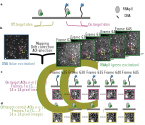
\includegraphics[width=145mm]{figures/figure1/figure1.png}
\caption{\textbf{Example CoSMoS experiment.} Data set A in Extended Data Table 1. \textbf{a}, Experiment schematic. DNA target molecules labeled with a blue-excited fluorescent dye (blue star) are tethered to the microscope slide surface. RNA polymerase II (RNApII) binder molecules labeled with a green-excited dye (green star) are present in solution. \textbf{b}, Data collection and preprocessing. After collecting a single image with blue excitation to identify the location of the DNA molecules, a time sequence of RNApII images were collected with green excitation.  Preprocessing of the images includes mapping of the corresponding points in target and binder channels, drift correction, and identification of two sets of areas of interest (AOIs).  One set corresponds to locations of target molecules (e.g., purple square); the other corresponds to locations where no target is present (e.g., yellow square). \textbf{c}, On-target data. Data are time sequences of $14 \times 14$ pixel AOI images centered at each target molecule. Frames show on-target (e.g., frame 630) and off-target (e.g., frame 645) binding of RNApII molecules. \textbf{d}, Off-target control data. Control data consists of images collected from randomly selected sites at which no target molecule is present. }
\label{fig:cosmos_experiment}
\end{figure}

% figure 2
\begin{figure}[h]
\centering
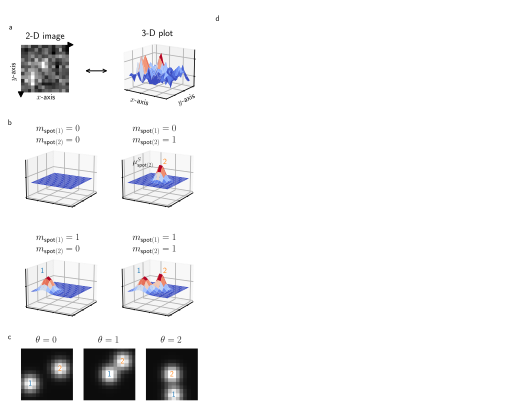
\includegraphics[width=\textwidth]{figures/figure2.png}
\label{fig:tapqir_model}
\caption{\textbf{Depiction of the probabilistic image model and model parameters.} \textbf{a}, Example AOI image from the Rpb1\textsuperscript{SNAP549} experimental data set. The AOI image is a matrix of $14 \times 14$ pixel intensities which is shown here as both a 2-D grayscale image and as a 3-D intensity plot. The image contains two spots, one is centered at target location (image center) and the other is located off-target. \textbf{b}, Examples of four idealized noise-free image representations ($\mu^I$). Image representations consist of zero, one, or two idealized spots ($\mu^S$) superimposed on a constant background ($b$). Each fluorescent spot is represented as a 2-D Gaussian parameterized by integrated intensity ($h$), width ($w$), and position ($x$, $y$). The presence of spots is encoded in the binary spot existence indicator $m$. \textbf{c}, Simulated idealized images illustrating different values of the target-specific spot index parameter $\theta$. $\theta = 0$ corresponds to a case when no specifically bound molecule is present; $\theta = 1$ or 2 corresponds to the cases in which the specifically bound molecule is spot 1 or 2, respectively. \textbf{d}, Condensed graphical representation of the probabilistic model. Model parameters are depicted as circles and deterministic functions as diamonds. Observed image ($D$) is represented by a shaded circle. Related nodes are connected by edges, with an arrow pointing towards the dependent node (e.g., the shape of each 2-D Gaussian spot $\mu^S$ depends on spot parameters $h$, $w$, $x$, and $y$). Plates (rounded rectangles) contain entities that are repeated for the number of instances displayed at the bottom-right corner: number of AOIs ($N$), frame count ($F$), and/or maximum number of spots in a single image ($K=2$). Parameters outside of the plates are global quantities that apply to all frames of all AOIs. A more complete version of the graphical model specifying the relevant probability distributions is given in Extended Data Fig. 1a. }
\end{figure}

% figure 3
\begin{figure}[h]
\centering
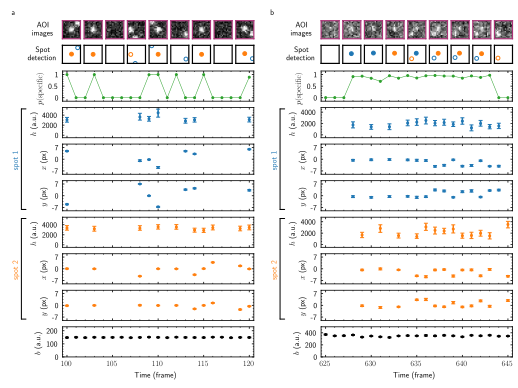
\includegraphics[width=\textwidth]{figures/figure3.png}
\caption{\textbf{Tapqir analysis and inferred model parameters.} \textbf{a},\textbf{b}, Tapqir was applied to simulated data (lamda0.5 parameter set in Supplementary Data 1) (\textbf{a}) and to experimental data (Data set A in Extended Data Table 1) (\textbf{b}). (\textbf{a}) and (\textbf{b}) each show a short extract from a single target location in the corresponding data set. The first row shows AOI images for the subset of frames indicated by gray shaded stripes in the plots. The second row shows the locations of spots determined by Tapqir. Only data for spots with a spot probability $p(m=1) > 0.5$ are shown. Spots predicted to be target-specific ($p(\theta=k)>0.5$ for spot $k$) are shown as filled circles. The graphs show the probability of there being any target-specific spot in a frame ($p(\mathsf{specific})$; green), spot intensity ($h$), location ($x$, $y$) of spot 1 (blue) and spot 2 (orange), and AOI background intensity ($b$). Error bars: 95\% CI (credible interval).  }
\label{fig:tapqir_analysis}
\end{figure}

% figure 4
\begin{figure}[h]
\centering
\includegraphics[width=\textwidth]{figures/figure4.png}
\caption{\textbf{Reproduction of experimental data by posterior predictive sampling.} Example frames are shown from Data set A  (\textbf{a}: $\mathrm{SNR}=1.63$), Data set B (\textbf{b}: $\mathrm{SNR}=3.43$), Data set C (\textbf{c}: $\mathrm{SNR}=4.18$), and Data set D (\textbf{d}: $\mathrm{SNR}=4.85$) in Extended Data Table 1. In each panel the top row shows AOI images selected from the experimental data and middle row shows corresponding images simulated by sampling from the posterior distributions. The bottom row shows pixel intensity distributions from the experimental and posterior prediction images shown. }
\label{fig:posterior_samples}
\end{figure}
\clearpage
\newpage

% figure 5
\begin{figure}[h]
\centering
\includegraphics[width=1\textwidth]{figures/figure5.png}
\caption{\textbf{Tapqir performance on simulated data with different SNRs or different non-specific binding rates.} \textbf{a-d}, Analysis of simulated data over a range of SNR. SNR was varied in the simulations by changing spot intensity  $h$ while keeping other parameters constant (Supplementary Data 3). \textbf{a}, Example images showing the appearance of the same target-specific spot simulated with increasing SNR.   \textbf{b}, Mean of Tapqir-calculated target-specific spot probability $p(\mathsf{specific})$ (with 95\% high-density region) for the subset of images where target-specific spots  are known to be present. \textbf{c}, Histograms of $p(\mathsf{specific})$ for selected simulations with SNR indicated. Data are shown as stacked bars for images known to have (green, 15\%) or not have (gray, 85\%) target-specific spots.  Count is zero for bins where bars are not shown. \textbf{d}, Accuracy of Tapqir image classification with respect to presence/absence of a target-specific spot. Accuracy was assessed by MCC, recall, and precision (see Text and Methods). \textbf{e-g}, Same as in (\textbf{b-d}) but for the data simulated over a range of non-specific binding rates $\lambda$ at fixed SNR = 3.76 (Supplementary Data 1). \textbf{h}, Same as in (\textbf{c}) but for the data simulated over a range of non-specific binding rates $\lambda$ with no target-specific binding ($\pi = 0$) (Supplementary Data 4).}
\label{fig:tapqir_performance}
\end{figure}

% figure 6
% move dots in between sample1 2
\begin{figure}[h]
\centering
\includegraphics[width=\textwidth]{figures/figure6.png}
\caption{\textbf{Tapqir analysis of association/dissociation kinetics and thermodynamics.} \textbf{a} Chemical scheme for a one-step association/dissociation reaction at equilibrium with apparent first-order binding and dissociation rate constants $k_{\mathrm{on}}$ and $k_{\mathrm{off}}$, respectively. \textbf{b}, A simulation of the reaction in (\textbf{a}) and scheme for kinetic analysis with Tapqir. Simulation used $\mathrm{SNR} = 3.76$, $k_\mathrm{on} = 0.02$ s$^{-1}$, $k_\mathrm{off} = 0.2$ s$^{-1}$, and a high target-nonspecific binding frequency $\lambda = 1$ (Supplementary Data 5, dataset kon0.02lambda1). Full dataset consists of 100 AOI locations and 1000 frames each for on-target data and off-target control data. Shown is a short extract of on-target data from a single location in the simulation.  Plots show simulated presence/absence of the target-specific spot (purple) and Tapqir-calculated estimate of corresponding target-specific spot probability $p(\mathsf{specific})$ (green). One thousand binary traces (e.g., black records) were sampled from the $p(\mathsf{specific})$ posterior distribution and used to infer $k_\mathrm{on}$ and $k_\mathrm{off}$ using a two-state hidden Markov model (HMM) (see Methods). Each sample trace contains well-defined time intervals corresponding to target-specific spot presence and absence (e.g., $\Delta t_\mathrm{on}$ and $\Delta t_\mathrm{off}$). \textbf{c,d,e}, Kinetic and equilibrium constants from simulations (Supplementary Data 5) using a range of $k_\mathrm{on}$ values and  target-nonspecific spot frequencies $\lambda$, with constant $k_\mathrm{off} = 0.2$ s$^{-1}$. \textbf{c} Values of $k_{\mathrm{on}}$ used in simulations (blue) and mean values (and 95\% CIs, black) inferred by HMM analysis from the 2000 posterior samples. \textbf{d}, Same as (\textbf{c}) but for $k_{\mathrm{off}}$. \textbf{e},  Binding equilibrium constants $K_{\mathrm{eq}} = k_{\mathrm{on}} / k_{\mathrm{off}}$ used in simulation (blue) and inferred from Tapqir-calculated $\pi$ as $K_{\mathrm{eq}} = \pi / (1 - \pi)$ (black). }
\label{fig:kinetic_analysis}
\end{figure}
\clearpage
\pagebreak

% figure 7
% add to Methods how CI is calculated
\begin{figure}[h]
\centering
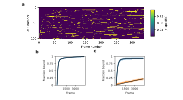
\includegraphics[width=\textwidth]{figures/figure7.png}
\caption{\textbf{Extraction of target-binder association kinetics from example experimental data.} Data are from Data set B (see Extended Data Table 1).  \textbf{a}, Probabilistic rastergram representation of Tapqir-calculated target-specific spot  probabilities $p(\mathsf{specific})$ (color scale). AOIs were ordered by decreasing times-to-first-binding. For clarity, only every thirteenth frame is plotted. \textbf{b}, Time-to-first-binding distribution using Tapqir. Plot shows the cumulative fraction of AOIs that exhibited one or more target-specific binding events by the indicated frame number (green) and fit curve (black). Shading indicates uncertainty. \textbf{c} Time-to-first-binding distribution using an empirical spot-picker method \cite{Friedman2013-sf}. The spot-picker method jointly fits first spots observed in off-target control AOIs (orange) and in on-target AOIs (blue) with fit curves (black). \textbf{d}, Values of kinetic parameters  $k_\mathrm{a}$, $k_\mathrm{ns}$, and $A_\mathrm{f}$ (see text) derived from fits in \textbf{b} and \textbf{c}. Uncertainties reported in (\textbf{b, c, d}) represent 95\% credible intervals for Tapqir and 95\% confidence intervals for spot-picker (see Methods).
}
\label{fig:experimental_data}
\end{figure}

% \clearpage
\newpage
\section*{Extended Data}
\pagebreak

\renewcommand{\figurename}{Extended Data Fig.}
\renewcommand{\tablename}{Extended Data Table}
% \renewcommand{\thetable}{S\arabic{table}}
\setcounter{figure}{0}

\begin{figure}[t]
\centering
\includegraphics[width=\textwidth]{extended-data/figure1/figure1.png}
\label{fig:full_model}
\end{figure}

%\addtocounter{figure}{-1}
\begin{figure} [t]
\caption{\textbf{Extended graphical representation of the generative probabilistic model and the prior distributions for $x$ and $y$ spot position parameters.} \textbf{a}, Directed factor graph representation \cite{Bishop2006-oa} of model parameters and parameter distributions. Model parameters are depicted as circles, parameter distributions as small filled squares, and deterministic functions as diamonds. Names of the probability distributions are written next to the squares. Input parameters and output parameters are connected by lines, with an arrow pointing towards the dependent parameter. Observed image ($D$) is the sum of the noisy photon-dependent image ($I$) and the photon-independent camera offset ($\delta$). Plates (rounded rectangles) contain nodes that are repeated for the number of instances displayed at the bottom-right corner: number of AOIs ($N$), frame count ($F$), maximum number of spots in a single image ($K$), and number of image pixels ($P \times P$). \textbf{b}, Prior distributions of $x$ and $y$ for specific and non-specific binding. Probability densities for $x$ and $y$ are defined in the range $\left[ -(P+1)/2, (P+1)/2 \right] $ relative to the target molecule and are conditional on the identity of the spot (specific or non-specific).  Probability densities for $x$ and $y$ parameters are identical. }
\end{figure}
%have a row above each data set with an experiment description, align columns
\clearpage

\begin{figure}[h]
\centering
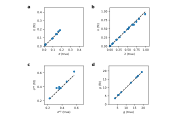
\includegraphics[width=\textwidth]{extended-data/figure2/figure2.png}
\caption{\textbf{Tapqir analysis and inferred spot probabilities.} \textbf{a},\textbf{b}, Tapqir was applied to simulated data (lamda0.5 parameter set in Supplementary Data 1) (\textbf{a}) and to experimental data (Rpb1\textsuperscript{SNAP549} in Extended Data Table 1) (\textbf{b}). (\textbf{a}) and (\textbf{b}) each show a short extract from a single target location in the corresponding data set. The first row shows AOI images for the subset of frames indicated by gray shaded stripes in the plots. The second row shows the locations of spots determined by Tapqir. Only data for spots with a spot probability $p(m=1) > 0.5$ are shown. Spots predicted to be target-specific ($p(\theta=k)>0.5$ for spot $k$) are shown as filled circles. The graphs show the probability of there being any target-specific spot in a frame ($p(\mathsf{specific})$; green), probability of being a target-specific spot ($p(\theta)$), probability of spot presence ($p(m=1)$) of spot 1 (blue) and spot 2 (orange).  }
\end{figure}
\pagebreak

% extended figure 3
\begin{figure}[h]
\centering
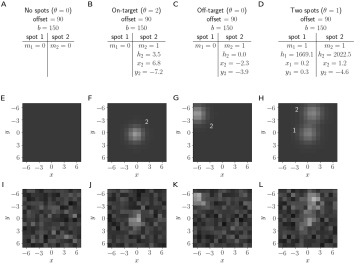
\includegraphics[width=\textwidth]{extended-data/figure3/figure2.png}
\caption{\textbf{Tapqir analysis of image data simulated using a broad range of global parameters.} Simulations (see Methods) consist of 16 datasets where values of global parameters ($\pi$, $\lambda$, $\sigma^{xy}$, and $g$) where randomly generated for each dataset (Supplementary Data 2). Simulated data were fit with Tapqir, and parameter values from the fit (with 95\% CI) are plotted against the true parameter values. To guide the eye, dashed lines  indicate identical true and fit values. \textbf{a}, Average specific binding probability $\pi$. \textbf{b}, Nonspecific binding rate $\lambda$. \textbf{c}, Proximity parameter $\sigma^{xy}$. \textbf{d}, Gain of the camera $g$. }
\label{fig:tapqir_global}
\end{figure}
\pagebreak

% extended figure 4
\begin{figure}[t]
\centering
\includegraphics[width=\textwidth]{extended-data/figure4.png}
\caption{\textbf{Additional example showing extraction of target-binder association kinetics from experimental data.} Data are from Data set A (see Extended Data Table 1).  Results are plotted as in Fig. 7, except that for clarity only every $2^\mathrm{nd}$ frame and every $3^\mathrm{rd}$ AOI is shown in \textbf{a}.

%Probabilistic rastergram representation of Tapqir-calculated target-specific spot  probabilities $p(\mathsf{specific})$ (color scale). AOIs were ordered by decreasing times-to-first-binding. For clarity, only every $2^\mathrm{nd}$ frame and every $3^\mathrm{rd}$ AOI is shown. \textbf{b,c}, Determining the association kinetic parameters [95\% CI] by  time-to-first-binding analysis using Tapqir (\textbf{b}) and an empirical spot-picker method \cite{Friedman2013-sf}(\textbf{c}).   Cumulative fraction of target sites that exhibited one or more binding events by the indicated frame number (blue) and fit curve (black) yielding best-fit values for $k_\mathrm{a}$, $k_\mathrm{ns}$, and $A_\mathrm{f}$. Shading indicates 95\% CI. Fitting protocol is different for the two methods; the spot-picker method fits both the target sites and off-target control data (orange) whereas Tapqir incorporates the control data in its $p(\mathsf{specific})$ calculation. \textbf{d}, Fit parameters. Error bars represent 95\% credible interval for Tapqir and 95\% confidence interval for spot-picker.
}
\label{fig:rpb1snap549}
\end{figure}
\pagebreak

% extended figure 5
\begin{figure}[t]
\centering
\includegraphics[width=\textwidth]{extended-data/figure5.png}
\caption{\textbf{Kinetic analysis of experimental data.} Data set C in Extended Data Table 1.  \textbf{a}, Probabilistic rastergram representation of Tapqir-calculated target-specific spot  probabilities $p(\mathsf{specific})$ (color scale). AOIs were ordered by decreasing times-to-first-binding. For clarity, only every $10^\mathrm{th}$ frame is shown. \textbf{b,c}, Determining the association kinetic parameters [95\% CI] by  time-to-first-binding analysis using Tapqir (\textbf{b}) and an empirical spot-picker method \cite{Friedman2013-sf}(\textbf{c}).   Cumulative fraction of target sites that exhibited one or more binding events by the indicated frame number (blue) and fit curve (black) yielding best-fit values for $k_\mathrm{a}$, $k_\mathrm{ns}$, and $A_\mathrm{f}$. Shading indicates 95\% CI. Fitting protocol is different for the two methods; the spot-picker method fits both the target sites and off-target control data (orange) whereas Tapqir incorporates the control data in its $p(\mathsf{specific})$ calculation. \textbf{d}, Fit parameters. Error bars represent 95\% credible interval for Tapqir and 95\% confidence interval for spot-picker.
}
\label{fig:sigma54_298P2993}
\end{figure}
\clearpage
\pagebreak


% extended figure 6
\begin{figure}[t]
\centering
\includegraphics[width=\textwidth]{extended-data/figure6.png}
\caption{\textbf{Kinetic analysis of experimental data.} Data set D in Extended Data Table 1.  \textbf{a}, Probabilistic rastergram representation of Tapqir-calculated target-specific spot  probabilities $p(\mathsf{specific})$ (color scale). AOIs were ordered by decreasing times-to-first-binding. For clarity, only every $13^\mathrm{th}$ frame is shown. \textbf{b,c}, Determining the association kinetic parameters [95\% CI] by  time-to-first-binding analysis using Tapqir (\textbf{b}) and an empirical spot-picker method \cite{Friedman2013-sf}(\textbf{c}).   Cumulative fraction of target sites that exhibited one or more binding events by the indicated frame number (blue) and fit curve (black) yielding best-fit values for $k_\mathrm{a}$, $k_\mathrm{ns}$, and $A_\mathrm{f}$. Shading indicates 95\% CI. Fitting protocol is different for the two methods; the spot-picker method fits both the target sites and off-target control data (orange) whereas Tapqir incorporates the control data in its $p(\mathsf{specific})$ calculation. \textbf{d}, Fit parameters. Error bars represent 95\% credible interval for Tapqir and 95\% confidence interval for spot-picker.
}
\label{fig:greb}
\end{figure}
\clearpage
\pagebreak

% clean up table formatting
% add how long it took to run
\begin{table}[h]
\caption{\label{tab:datasets} \textbf{Experimental data sets.}}
\resizebox{\textwidth}{!}{%
% Use "S" column identifier to align on decimal point 
\begin{tabular}{ccccccc}
\toprule
Data set size\textsuperscript{a} & SNR & $\pi$ & $\lambda$ & $g$ & $\sigma^{xy}$ & Compute time \\
\midrule
\multicolumn{7}{l}{\parbox{1.2\textwidth}{Data set A: Binder, SNAP\textsubscript{f}-tagged \textit{S. cerevisiae} RNA polymerase II labeled with DY549; Target, transcription template DNA containing $5 \times$ Gal4 upstream activating sequences and \textit{CYC1} core promoter; Conditions, yeast nuclear extract supplemented with Gal4-VP16 activator and NTPs. From \cite{Rosen2020-zn}.}} \\
\\
\begin{tabular}[x]{@{}c@{}}$N = 331$, $F = 790$\\$N_c = 526$, $F_c = 790$\end{tabular} & $1.6268$ &
$0.10217\:[0.10086, 0.10346]$ & $0.29576\:[0.29420, 0.29699]$ & $6.5069\:[6.5053, 6.5085]$ & $0.5537\:[0.5489, 0.5573]$ & 6 h \\
\midrule
\multicolumn{7}{l}{\parbox{\textwidth}{Data set B: Binder, 0.4 nM \textit{E. coli} $\sigma^{54}$ RNA polymerase labeled with Cy3; Target,  3,591 bp DNA containing the \textit{glnALG} promoter; Conditions, phyiological buffer, no NTPs. From (Fig. 3D) of \cite{Friedman2013-sf}.}} \\
\\
\begin{tabular}[x]{@{}c@{}}$N = 122$, $F = 3855$\\$N_c = 157$, $F_c = 3855$\end{tabular} & $4.1766$ & $0.02591\:[0.02529, 0.02649]$ & $0.07157\:[0.07073, 0.07223]$ & $16.6353\:[16.6297, 16.6406]$ & $0.3342\:[0.3307, 0.3370]$ & 5 h 45 m \\
\midrule
\multicolumn{7}{l}{\parbox{\textwidth}{Data set C: Binder, 0.1 nM \textit{E. coli} $\sigma^{54}$ RNA polymerase labeled with Cy3; Target, 852 bp DNA containing the \textit{glnALG} promoter; Conditions, phyiological buffer, no NTPs. From  (Fig. 1E) of \cite{Friedman2013-sf}.}} \\
\\
\begin{tabular}[x]{@{}c@{}}$N = 102$, $F = 4407$\\$N_c = 127$, $F_c = 4407$\end{tabular} & $3.4288$ & $0.08523\:[0.08420, 0.08627]$ & $0.12900\:[0.12795, 0.12985]$ & $11.7900\:[11.7854, 11.7945]$ & $0.4240\:[0.4214, 0.4261]$ & 8 h 20 m \\
\midrule
\multicolumn{7}{l}{\parbox{\textwidth}{Data set D: Binder, 0.15 nM \textit{E. coli} Cy3-GreB; Target, reconstituted backtracked EC-6 \textit{E. coli} transcription elongation complex; Conditions, phyiological buffer, no NTPs.  Subset of data set from \cite{Tetone2017-za}.}} \\
\\
\begin{tabular}[x]{@{}c@{}}$N = 100$, $F = 5622$\\$N_c = 100$, $F_c = 5622$\end{tabular} & $4.8479$ & $0.00297\:[0.00266, 0.00328]$ & $0.04040\:[0.03942, 0.04123]$ & $16.9710\:[16.9609, 16.9809]$ & $0.2954\:[0.2847, 0.3054]$ & 6h \\
\bottomrule
\multicolumn{7}{l}{\footnotesize{\parbox{\textwidth}{\textsuperscript{a}$N$ - number of on-target AOIs, $F$ - number of frames for on-target AOIs, $N_c$ - number of control off-target AOIs, $F_c$ - number of frames for off-target AOIs.}}} \rule{0pt}{3ex} \\
\end{tabular}}
\end{table}
\clearpage
\pagebreak



\begin{table}[h]
\caption{\label{tab:parameters} \textbf{Glossary of mathematical symbols.}}
\begin{tabular}{l l l}
\toprule
Symbol & Description & Domain \\
\midrule
$K$ & maximum number of spots per image & $\mathbb{N}$ \\
$N$ & number of AOIs & $\mathbb{N}$ \rule{0pt}{3ex} \\
$F$ & number of frames & $\mathbb{N}$ \rule{0pt}{3ex} \\
$P$ & number of pixels & $\mathbb{N}$ \rule{0pt}{3ex} \\
$g$ & camera gain & $\mathbb{R}_{>0}$ \rule{0pt}{3ex} \\
$\sigma^{xy}$ & proximity & $(0, (P+1)/\sqrt{12})$ \rule{0pt}{3ex} \\
$\pi$ & average target-specific binding probability & [0, 1] \rule{0pt}{3ex} \\
$\lambda$ & target-nonspecific binding rate & $\mathbb{R}_{>0}$ \rule{0pt}{3ex} \\
$\mu^b$ & mean background intensity across AOI & $\mathbb{R}_{>0}^{\mathsf{AOI}[N]}$ \rule{0pt}{3ex} \\
$\sigma^b$ & standard deviation of background intensity across AOI & $\mathbb{R}_{>0}^{\mathsf{AOI}[N]}$ \rule{0pt}{3ex} \\
$b$ & background intensity & $\mathbb{R}_{>0}^{\mathsf{AOI}[N] \times \mathsf{frame}[F]}$ \rule{0pt}{3ex} \\
$\theta$ & target-specific spot index & $\{0, 1, \dots, K \}^{\mathsf{AOI}[N] \times \mathsf{frame}[F]}$ \rule{0pt}{3ex} \\
$m$ & spot presence indicator & $\{ 0, 1 \}^{\mathsf{spot}[K] \times \mathsf{AOI}[N] \times \mathsf{frame}[F]}$ \rule{0pt}{3ex} \\
$h$ & integrated spot intensity & $\mathbb{R}_{>0}^{\mathsf{spot}[K] \times \mathsf{AOI}[N] \times \mathsf{frame}[F]}$ \rule{0pt}{3ex} \\
$w$ & spot width & $[0.75, 2.25]^{\mathsf{spot}[K] \times \mathsf{AOI}[N] \times \mathsf{frame}[F]}$ \rule{0pt}{3ex} \\
$x$ & center of the spot on the $x$-axis & $\mathbb{R}^{\mathsf{spot}[K] \times \mathsf{AOI}[N] \times \mathsf{frame}[F]}$ \rule{0pt}{3ex} \\
$y$ & center of the spot on the $y$-axis & $\mathbb{R}^{\mathsf{spot}[K] \times \mathsf{AOI}[N] \times \mathsf{frame}[F]}$ \rule{0pt}{3ex} \\
$\mu^S$ & 2-D Gaussian spot & $\mathbb{R}_{>0}^{\mathsf{spot}[K] \times \mathsf{AOI}[N] \times \mathsf{frame}[F] \times \mathsf{pixelX}[P] \times \mathsf{pixelY}[P]}$ \rule{0pt}{3ex} \\
$\mu^I$ & ideal image & $\mathbb{R}_{>0}^{\mathsf{AOI}[N] \times \mathsf{frame}[F] \times \mathsf{pixelX}[P] \times \mathsf{pixelY}[P]}$ \rule{0pt}{3ex} \\
$\delta$ & offset signal & $\mathbb{R}_{>0}^{\mathsf{AOI}[N] \times \mathsf{frame}[F] \times \mathsf{pixelX}[P] \times \mathsf{pixelY}[P]}$ \rule{0pt}{3ex} \\
$I$ & observed image w/o offset & $\mathbb{R}_{>0}^{\mathsf{AOI}[N] \times \mathsf{frame}[F] \times \mathsf{pixelX}[P] \times \mathsf{pixelY}[P]}$ \rule{0pt}{3ex} \\
$D$ & observed image & $\mathbb{R}_{>0}^{\mathsf{AOI}[N] \times \mathsf{frame}[F] \times \mathsf{pixelX}[P] \times \mathsf{pixelY}[P]}$ \rule{0pt}{3ex} \\
$x^\mathsf{target}$ & target molecule position on the $x$-axis & $[P/2-1, P/2]^{\mathsf{AOI}[N] \times \mathsf{frame}[F]}$ \rule{0pt}{3ex} \\
$y^\mathsf{target}$ & target molecule position on the $y$-axis & $[P/2-1, P/2]^{\mathsf{AOI}[N] \times \mathsf{frame}[F]}$ \rule{0pt}{3ex} \\
$i$ & pixel index on the $x$-axis & $\{0, \dots, (P-1)\}^{\mathsf{pixelX}[P]}$ \rule{0pt}{3ex} \\
$j$ & pixel index on the $y$-axis & $\{0, \dots, (P-1)\}^{\mathsf{pixelX}[P]}$ \rule{0pt}{3ex} \\
$D^\mathsf{raw}$ & raw microscope images & $\mathbb{R}_{>0}^{\mathsf{frame}[F] \times \mathsf{pixelX}[H] \times \mathsf{pixelY}[W]}$ \rule{0pt}{3ex} \\
$x^{\mathsf{target}, \mathsf{raw}}$ & target molecule position in raw images on the $x$-axis & $[-0.5, H-0.5]^{\mathsf{AOI}[N] \times \mathsf{frame}[F]}$ \rule{0pt}{3ex} \\
$y^{\mathsf{target}, \mathsf{raw}}$ & target molecule position in raw images on the $y$-axis & $[-0.5, W-0.5]^{\mathsf{AOI}[N] \times \mathsf{frame}[F]}$ \rule{0pt}{3ex} \\
\bottomrule
\end{tabular}
\end{table}
\clearpage
\pagebreak

\begin{table}[h]
\caption{\label{tab:dist} \textbf{Probability distributions used in the model.}}
\begin{tabular}{l l}
\toprule
Distribution & PDF \\
\midrule
$x \sim \mathbf{AffineBeta}(\mu, \nu, a, b)$ &
    $\dfrac{y^{\alpha-1}(1-y)^{\beta-1}}{\text{B}(\alpha, \beta)}$
    where $\alpha=\dfrac{\nu (\mu-a)}{b-a}$, $\beta=\dfrac{\nu (b-\mu)}{b-a}$, and $y = \dfrac{x-a}{b-a}$ \\
$x \sim \mathbf{Bernoulli}(\pi)$ &
    $\pi^x (1-\pi)^{1-x}$ \\
$x \sim \mathbf{Beta}(\alpha, \beta)$ &
    $\dfrac{x^{\alpha-1}(1-x)^{\beta-1}}{\text{B}(\alpha, \beta)}$ \\
$x \sim \mathbf{Categorical}_{\{z_i\}^k_{i=1}}(\mathbf{p})$ &
    $\prod_{i=1}^k p_i^{[x=z_i]}$ \\
$x \sim \mathbf{Gamma}(\mu, \sigma)$ &
    $\dfrac{\beta^\alpha}{\Gamma(\alpha)}x^{\alpha-1} e^{-\beta x}$
    where $\alpha = \dfrac{\mu^2}{\sigma^2}$ and $\beta = \dfrac{\mu}{\sigma^2}$ \\
$x \sim \mathbf{HalfNormal}(\sigma)$ &
    $\dfrac{\sqrt{2}}{\sigma \sqrt{\pi}} \exp \left( -\dfrac{x^2}{2\sigma^2} \right)$
    for  $x > 0$ \\
$k \sim \mathbf{TruncatedPoisson}(\lambda, K) $ & $ \begin{cases} 1 - e^{-\lambda} \sum_{i=0}^{K-1} \dfrac{\lambda^i}{i!} & \textrm{if $k = K$} \\ \dfrac{\lambda^k e^{-\lambda}}{k!} & \textrm{otherwise} \end{cases} $ \\
$x \sim \mathbf{Uniform}(a, b)$ &
    $\dfrac{1}{b-a}$ for $x \in [a, b]$ \\
\bottomrule
\end{tabular}
\end{table}

\section{Supplemental Data}

\begin{itemize}
    \item \textbf{Supplemental Data 1: Varying non-specific binding rate simulation parameters and corresponding fit values.}

    \item \textbf{Supplemental Data 2: Randomized simulation parameters and corresponding fit values.}

    \item \textbf{Supplemental Data 3: Varying intensity (SNR) simulation parameters and corresponding fit values.}

    \item \textbf{Supplemental Data 4: No target-specific binding and varying non-specific binding rate simulation parameters and corresponding fit values.}

    \item \textbf{Supplemental Data 5: Kinetic simulation parameters and corresponding fit values.}
    
    \item \textbf{Supplemental Data 6: Varying proximity simulation parameters and corresponding fit values.}
\end{itemize}

\end{document}